\input preamble.tex

\startEntry{}
\section{Mathematical eggs}
How many eggs should you eat? Who knows. All I know is that I want an excuse to have some more images and formulae and things.
Let's draw a fuction.
\section{The Egg equation}
The quality of a cooked egg varies with the time taken to cook it. X is in minutes and Y is tastiness. A good approximation for this is \[x^3 - 6x^2 + 11x - 4\] for $x \in [1/2, 5/2]$.
This function looks a bit like this in the region we want to consider:
\begin{figure}[h]
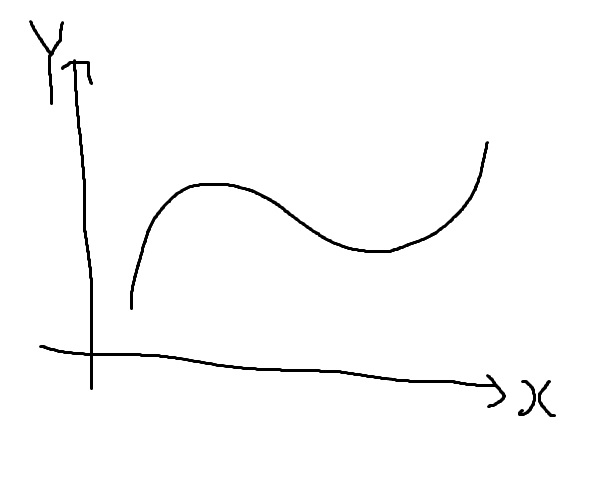
\includegraphics[height = 7cm]{simple_graph.jpg}
\end{figure}

Next time we will analyse this function and try to find a good way to cook the egg.
\finishEntry{}